\documentclass{article}
\usepackage{amsmath}
\usepackage{mathtext}
\usepackage[T1,T2a]{fontenc}
\usepackage[utf8]{inputenc}
\usepackage[english, bulgarian, russian]{babel}
\usepackage{tikz}
\usepackage{pgfplots}
\usepackage[export]{adjustbox}
\usepackage[left=2cm,right=2cm,
    top=2cm,bottom=2cm,bindingoffset=0cm]{geometry}

\title{Изучение электронного осциллографа}
\date{2019-09-30}
\author{Панферов Андрей}

\begin{document}
\topmargin=-10mm
\pagenumbering{gooble}
\maketitle
\newpage
\pagenumbering{arabic}

\section{Устройство осциллографа:}

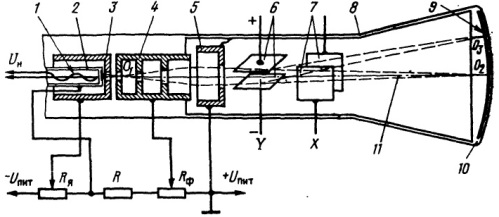
\includegraphics[width=1\textwidth]{osci.jpg}


\section{Наблюдение периодического сигнала от генератора и измерение его частоты.}
\begin{table}[h!]
\begin{center}
\caption{Измерения частот сигнала}
\begin{tabular}{|c|c|c|c|c|c|c|}
	\hline
	$f_{ЗГ}$, Гц & T, дел & с/дел & T, сек & f, Гц & $\delta f$, Гц & $f-f_{ЗГ}$, Гц \\
	\hline
	 199 & 5.2 & $1\cdot10^{-3}$ & $5.2\cdot10^{-3}$ & 192 & 8 & 7 \\
	\hline
	 1000 & 5.0 & $0.2\cdot10^{-3}$ & $1\cdot10^{-3}$ & 1000 & 40 & 0 \\
	\hline
	 1997 & 5.0 & $0.1\cdot10^{-3}$ & $0.5\cdot10^{-3}$ & 2000 & 80 & 3 \\
	\hline
	 3000 & 6.8 & $50\cdot10^{-6}$ & $0.34\cdot10^{-3}$ & 2941 & 90 &  60\\
	\hline
	 5000 & 4.2 & $50\cdot10^{-6}$ & $0.21\cdot10^{-3}$ & 4762 & 230 & 240 \\
	\hline
\end{tabular}
\end{center}
\end{table}

\section{Измерение амплитуды сигнала.}
\begin{align*}
U_{MAX} =& 11В&
	U_{MIN} =& 12мВ& \\
2.2дел;\: \: & 5\frac{В}{дел}&
	2.4дел;\: \: & 5\frac{мВ}{дел}& \\
\frac{\delta U_{MAX}}{U_{MAX}} \approx& 0.09& 
	 \frac{\delta U_{MIN}}{U_{MIN}} \approx& 0.09& 
\end{align*}



\begin{equation*}
\beta_{21}[дБ]=10\lg\frac{P_2}{P_1}=20\lg\frac{U_2}{U_1}=59.24дБ \: \: \: \: \delta \beta_{21} \approx 0.13
\end{equation*}

где $\frac{P_2}{P_1}$ — отношение средних мощностей,$\frac{U_2}{U_1}$ — отношениеамплитуд некоторых двух сигналов (здесь учтено, что мощностьпопорциональна квадрату амплитуды $P \sim U^2$).

\newpage

\section{Измерение амплитудно-частотной характеристики осциллографа.}

Измерим амплитудно-частотную характеристику K(f) при открытом (DC,$\:\approx$) и при закрытом (AC,$\:\sim$) входе. Результаты занесeм в таблицу 2.

\begin{table}[h!]
\begin{center}
\caption{Амплитудно-частотная характеристика $K(f)$}
\begin{tabular}{|c|c|c|c|c|c|c|c|c|}
\hline
f,Гц&1.3&5.0&10.0&100&1000&10000&$1 \cdot 10^6$&$5 \cdot 10^6$ \\
\hline
$\lg f$&0.11&0.7&1.0&2.0&3.0&4.0&6.0&6.7 \\
\hline
$2U_{ac}$, дел&2.0&5.0&5.6&6.0&6.0&6.0&6.0&5.6 \\
\hline
$K_{AC} = \frac{U_{AC}}{U_0}$&0.33&0.83&0.93&1.0&1.0&1.0&1.0&0.93 \\
\hline
$2U_{DC}$,дел&6.0&6.0&6.0&6.0&6.0&6.0&6.0&6.3 \\
\hline
$K_{DC} = \frac{U_{DC}}{U_0}$&1.0&1.0&1.0&1.0&1.0&1.0&1.0&0.93 \\
\hline
\end{tabular}
\end{center}
\end{table}

\begin{tikzpicture}[scale = 1.33]
\begin{axis}[
    axis lines = left,
    legend style={at={(0.1,-0.1)}},
    xlabel = {$\lg f$},
    ylabel = {K},
    xmin=0, xmax=7,
    ymin=0, ymax=1.1,
	ymajorgrids = true,
	xmajorgrids = true
]
\addplot[
	mark = square, 
	mark options = {
		scale = 1.5, 
		fill = red, 
		draw = chucknorris
	},
	ymajorgrids = true,
	xmajorgrids = true,
	color = blue 
]  coordinates {
	(0.11,0.33) (0.7,0.83) (1,0.93) (2,1.0) (3,1.0) (4,1.0) (6,1.0) (6.7,0.93)};
\addplot[
	mark = triangle, 
	mark options = {
		scale = 1.5, 
		fill = blue, 
		draw = chucknorris
	},
	ymajorgrids = true,
	xmajorgrids = true,
	color = red
] coordinates {
	(0.11,1) (0.7,1) (1,1) (2,1) (3,1) (4,1) (6,1) (6.7,0.93)};
\legend{ 
	$K_{DC}$, 
	$K_{AC}$
};

\end{axis}
\end{tikzpicture}

$\:$

Вероятной причиной различия АЧХ осциллографа в разных режимах является емкость, включающаяся в схему осциллографа в режиме DC. При больших частотах ее импеданс становится мал, и почти не влияет на показания прибора, но на маленьких частотах он становится значительным и способен изменить показания
$\:$

\section{}
$\:$
\section{Измерение разности фазово-частотных характеристик каналов осциллографа.}

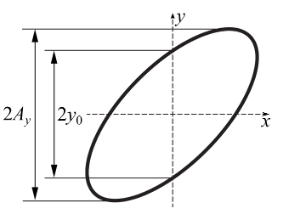
\includegraphics[width=1\textwidth]{osci.png}

При подаче на взаимно перпендикулярные отклоняющие пла-стины двух синусоидальных сигналов траектория луча на экранеосциллографа представляет собой эллипс и может быть в общемвиде описана уравнениями:

\begin{equation}
\left. x(t) = A_x \sin{\omega t + \Phi_x}, \right y(t) = A_y \sin{\omega t + \Phi_y}
\begin{equation}

Разность фаз $\delta\Phi = \Phi_y - \Phi_x$ можно выразить, например, положив $\omega t = -\Phi_x$, после чего нетрудно получить: 
$\:sin|\delta\Phi| = |\frac{y_0}{A_y}|$

Тогда: 
\begin{equation*}
\delta\Phi = arcsin|\frac{y_0}{A_y}| \:\: или \:\: \delta\Phi = \pi - arcsin|\frac{y_0}{A_y}| \:\: или \:\: \delta\Phi = \pi + arcsin|\frac{y_0}{A_y}|


\end{equation*}

\begin{table}
\begin{center}
\caption{Фаза-частотная характеристика $\delta\Phi(f)$}
\begin{tabular}{|c|c|c|c|c|c|c|c|c|c|c|c|c|}
\hline
$f$, МГц&0.001&0.125&0.330&0.530&1.00&1.50&1.60&1.80&2.41&2.78&3.50&5.00\\
\hline
$\lg f$&3.00&5.10&5.52&5.72&6.00&6.17&6.20&6.25&6.41&6.44&6.54&6.70\\
\hline
$|2y_0|$, дел&0&0.4&1.2&2.0&4.0&6.0&6.2&7.6&6.0&4.0&0&6.70\\
\hline
$|2A_y|$, дел&7.6&7.6&7.6&7.6&7.6&7.6&7.6&7.6&7.6&7.6&7.4&7.2\\
\hline
$arcsin|\frac{y_0}{A_y}|$, рад&0&0.053&0.16&0.27&0.55&0.91&1.11&1.57&0.91&0.55&0&0.62\\
\hline
$|\delta\Phi|$, рад&0&0.05&0.16&0.27&0.55&0.91&1.11&1.57&2.23&2.59&3.14&3.76\\
\hline

\end{tabular}
\end{center}
\end{table}

\begin{tikzpicture}[scale = 1.7]
\begin{axis}[
    axis lines = left,
    legend style={at={(0.1,-0.1)}},
    xlabel = {$\lg f$},
    ylabel = {$\delta\Phi$},
    xmin=3, xmax=7,
    ymin=0, ymax=4,
	ymajorgrids = true,
	xmajorgrids = true
]
\addplot[
	mark = square, 
	mark options = {
		scale = 1.5, 
		fill = red, 
		draw = chucknorris,
	}
]  coordinates {
	(3,0)(5.10,0.05)(5.52,0.16)(5.72,0.27)(6.00,0.55)(6.17,0.91)(6.20,1.11)(6.25,1.57)(6.41,2.23)(6.44,2.59)(6.54,3.14)(6.70,3.76)};

\legend{ 
	$\delta\Phi$
};

\end{axis}
\end{tikzpicture}

\newpage

\section{Наблюдение фигур Лиссажу и измерение частоты.}

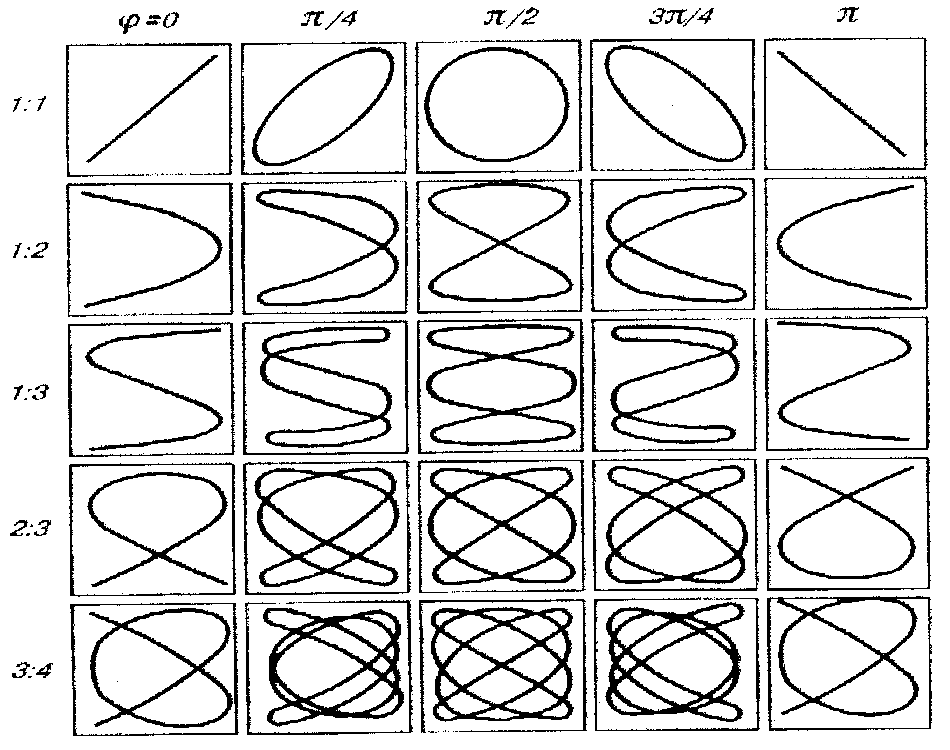
\includegraphics[width=1\textwidth]{lis.png}

\section{Измерение АЧХ интегрирующей и дифференцирующей RC-цепочек.}

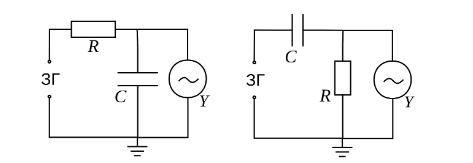
\includegraphics[width=1\textwidth]{schemes.png}


а) Интегрирующая» цепочка \: \:  б) «Дифференцирующая» цепочка

\begin{align*}
\left. K_a(f) =& \frac{1}{\sqrt{(\Omega \tau)^2 + 1}};& 
	\right K_б(f) =& \frac{1}{\sqrt{(\Omega \tau)^{-2} + 1}}& \\
R =& 3.0\cdot 10^{3} Ом;&
	C =& 0.01 \cdot 10^{-6} Ф& \\
\end{align*}



где $\tau = RC = 3.0 \cdot 10^{-5} c$ — постоянная времени RC-цепочки

\begin{table}[!h]
\begin{center}
\caption{АЧХ интегрирующей и дифференцирующей RC-цепочек}
\begin{tabular}{|c|c|c|c|c|c|}
\hline
$f$, Гц&$A_{in}$, дел&$A_{out}^{int}$,дел&$A_{out}^{def}$,дел&$K^{int}$&$K^{def}$\\
\hline
3.0&3.8&3.8&0&1&0\\
\hline
10&5.8&5.8&0&1&0\\
\hline
60&6.0&6.0&0&1&0\\
\hline
100&6.0&6.0&0&1&0\\
\hline
500&6.0&6.0&0.6&1&0.1\\
\hline
$2\cdot10^3$&6.0&5.6&2.0&0.93&0.33\\
\hline
$5\cdot10^3$&6.0&4.4&3.8&0.73&0.63\\
\hline
$10\cdot10^3$&6.0&3.0&5.1&0.50&0.85\\
\hline
$20\cdot10^3$&6.0&1.4&5.5&0.23&0.92\\
\hline
$30\cdot10^3$&6.0&1.1&5.6&0.18&0.93\\
\hline
$40\cdot10^3$&6.0&0.8&5.7&0.13&0.95\\
\hline
$50\cdot10^3$&6.0&0.7&5.8&0.12&0.97\\
\hline
$60\cdot10^3$&6.0&0.6&5.8&0.10&0.97\\
\hline
$70\cdot10^3$&6.0&0.5&5.8&0.08&0.97\\
\hline
\end{tabular}
\end{center}
\end{table}



\begin{tikzpicture}[scale = 1.5]
\begin{axis}[
    axis lines = left,
    legend style={at={(0.1,-0.1)}},
    xlabel = {$f$, Гц},
    ylabel = {$K$},
    xmin=0, xmax=75000,
    ymin=0, ymax=1.2,
	ymajorgrids = true,
	xmajorgrids = true
]
\addplot[
	mark = square, 
	mark options = {
		scale = 1.5, 
		fill = red, 
		draw = chucknorris
	}
]  coordinates {(3,1)(10,1)(60,1)(100,1)(500,1)(2000,0.93)(5000,0.73)(10000,0.5)(20000,0.23)(30000,0.18)(40000,0.13)(50000,0.12)(60000,0.1)(70000,0.08)
	};

\addplot[
	mark = triangle, 
	mark options = {
		scale = 1.5, 
		fill = red, 
		draw = chucknorris
	}
]  coordinates {(3,0)(10,0)(60,0)(100,0)(500,0.1)(2000,0.33)(5000,0.63)(10000,0.85)(20000,0.92)(30000,0.93)(40000,0.95)(50000,0.97)(60000,0.97)(70000,0.97)
	};

\legend{ 
	$K^{int}$,
	$K^{def}$
};

\addplot [
    domain=1:70000, 
    samples=50, 
    color=red,
]
{1/sqrt(1+(x*1.88*10^(-4))^2)};

\addplot [
    domain=1:70000, 
    samples=1000, 
    color=blue,
]
{1/sqrt(1+1/((x*1.88*10^(-4))^2))};



\end{axis}
\end{tikzpicture}

\begin{equation*}
\end{euqtion*}

Вывод: в этой работе мы научились работать с электронным осцилллографом в различных диапазонах измерений и режимах развертки, изучили методы его применения и нашли, в каких диапазонах входных данных его показаниям можно верить. Мы пронаблюдали фигуры Лиссажу.
\end{document}